\section{Simulation Analysis}
\label{sec:simulation}


\begin{table}[H]
  \centering
  \begin{tabular}{|l|r|}
    \hline    
    {\bf Voltages} & {\bf V} \\ \hline
    zin & 1.161859e+03\\ \hline

  \end{tabular}
  \caption{NPN Voltages and F.A.R confirmation}
  \label{tab1:npn}
\end{table}


\begin{table}[H]
  \centering
  \begin{tabular}{|l|r|}
    \hline    
    {\bf Voltages} & {\bf V} \\ \hline
    zout & 8.251525e+02\\ \hline

  \end{tabular}
  \caption{NPN Voltages and F.A.R confirmation}
  \label{tab2:npn}
\end{table}


\begin{table}[H]
  \centering
  \begin{tabular}{|l|r|}
    \hline    
    {\bf Voltages} & {\bf V} \\ \hline
    Gain(dB)&37.0419\\ \hline
Gain& 71.1371\\ \hline
Central Frequency(Hz)& 1051.2\\ \hline
Gain deviation&28.8629\\ \hline
Central frequency deviation(Hz)&51.2041\\ \hline
Cost(MU)& 13446.7\\ \hline
Merit & 9.28821E-07\\ \hline

  \end{tabular}
  \caption{NPN Voltages and F.A.R confirmation}
  \label{tab3:npn}
\end{table}

\begin{figure}[H] \centering
 \includegraphics[width=0.6\linewidth]{gain.pdf}
 \caption{Phase Frequency Response}                         %%%%%%%%%%LEGENDA
\label{fig:phase}
\end{figure}

\begin{figure}[H] \centering
 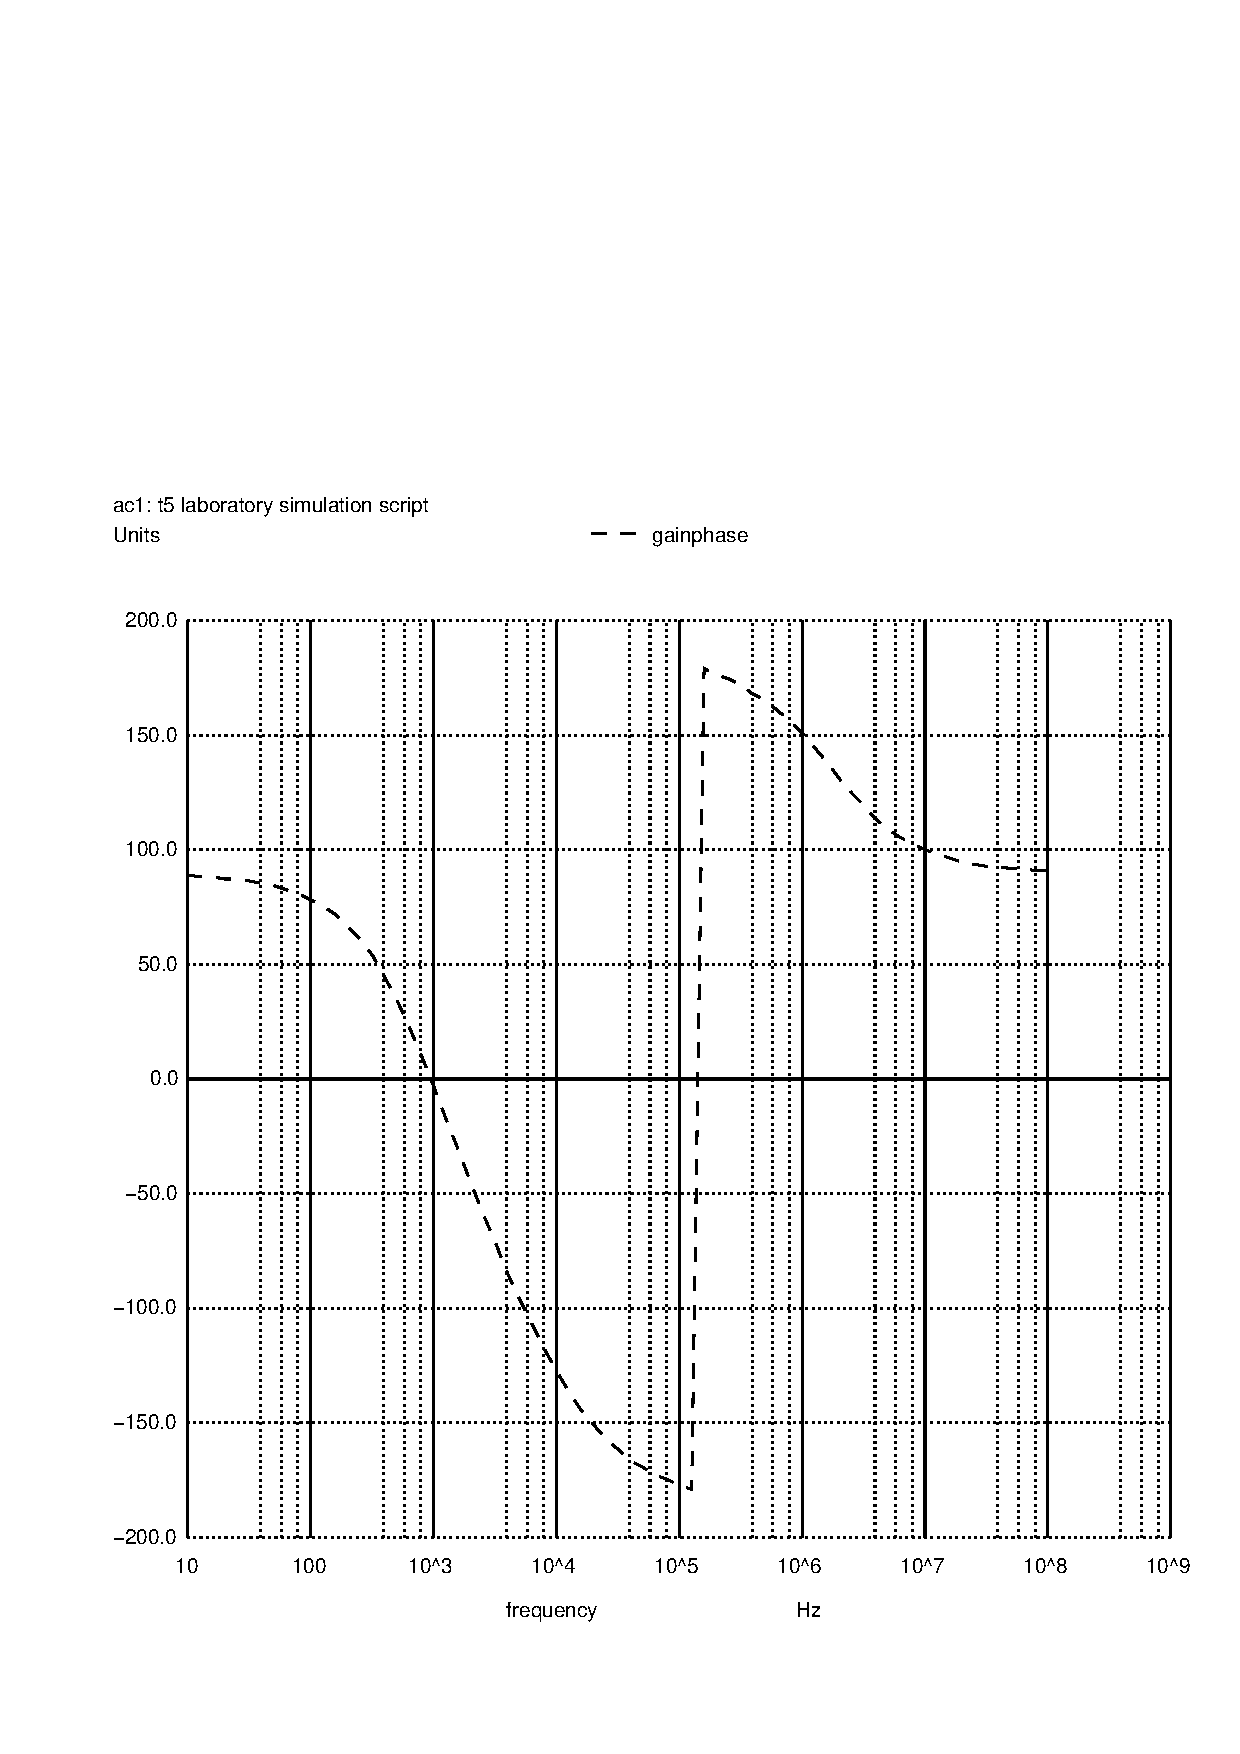
\includegraphics[width=0.6\linewidth]{phase.pdf}
 \caption{Phase Frequency Response}                         %%%%%%%%%%LEGENDA
\label{fig:phase}
\end{figure}

%\begin{table}[H]
%  \centering
%  \begin{tabular}{|l|r|}
%    \hline    
%    {\bf Name} & {\bf V or dB} \\ \hline
%    \input{../sim/sim_tab}
%  \end{tabular}
%  \begin{tabular}{|l|c|}
%    \hline
%    {\bf Impedance} & {\bf kOhms} \\ \hline
%    zin & 2.236262e+00\\ \hline

%  \end{tabular}
%  \begin{tabular}{|l|c|}
%    \hline
%    {\bf Impedance} & {\bf kOhms} \\ \hline
%    \input{../sim/output_tab2}
%  \end{tabular}
%    \caption{Simulation Results.}
%    \label{tab1:sim}
%\end{table}

It is important, in order to guarantee a high compatibility with AUDIO IN and speakers, that we obtain a very high input impedance ($Z_I$) and a very low output impedance ($Z_O$). Analysing our results, we notice that despite having a small input impedance (in result of a compromise we had to make to obtain a higher merit figure), the output impedance is very low, as desired.


\subsection{Coupling Capacitors}
In order to analyse this circuit, we need to understand the coupling capacitors influence. In this BJT amplifier circuit, there are two couplin capacitors, $C_{in}$ and $C_O$ - because their functions are similar, we will focus only on capacitor $C_{in}$. In the graphics below, we present the frequency response of the circuit, but with $C_{in}$ values drastically differents.

As we can notice, the change in the capacitance of the coupling capacitor does not influence the value of the higher cut-off frequency. However, the increase of that value leads to a larger bandwidth, which is desired.
\subsection{Gain.}
%\pagebreak
%\vspace{-2.5cm}

%\begin{figure}[h]
%\centering
%\begin{subfigure}{.5\textwidth}
%    \centering
%    \vspace{2.8 cm}
%    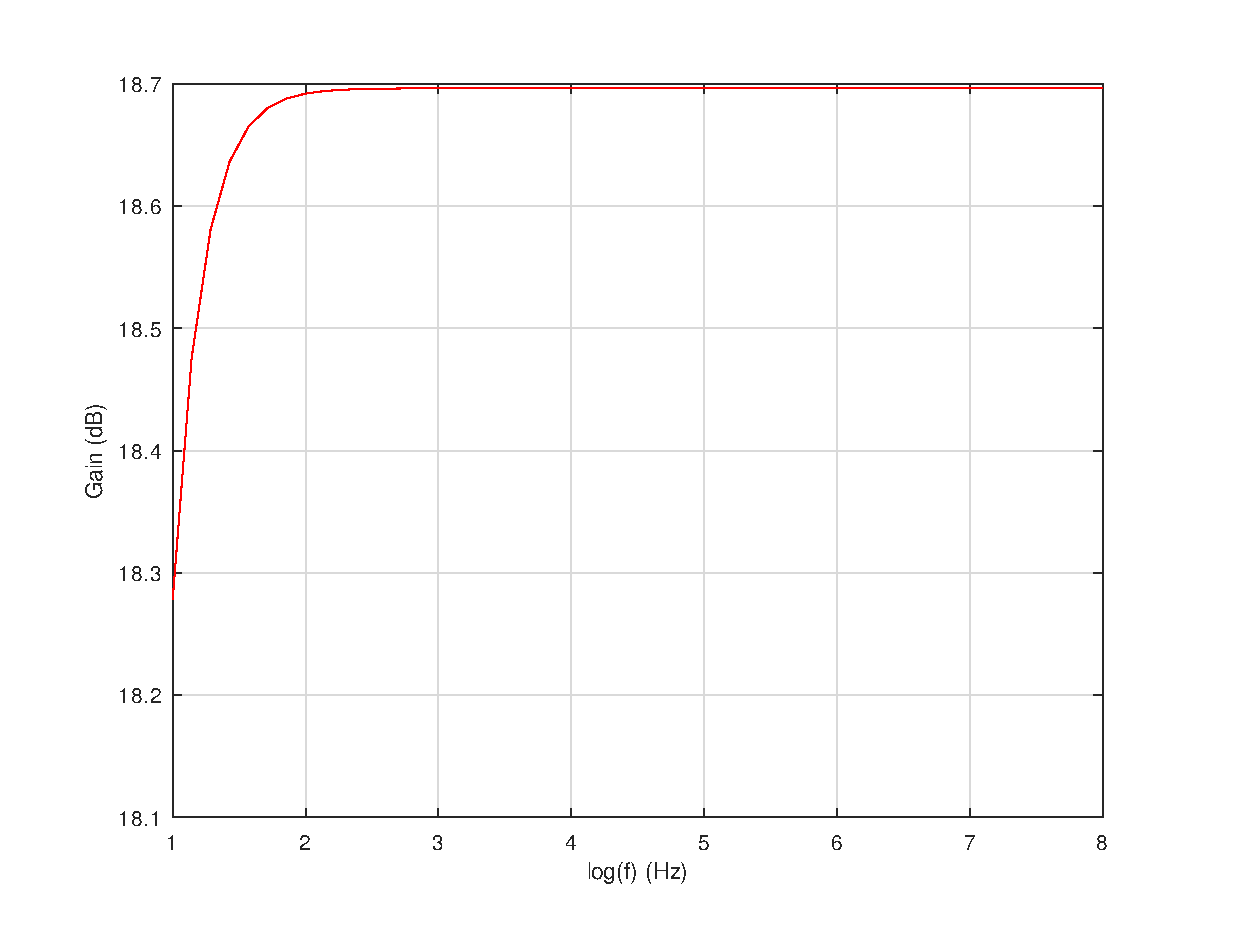
\includegraphics[scale=0.4]{Gain.eps}
%    \caption{Theoretical Gain}
%\end{subfigure}%
%\begin{subfigure}{.5\textwidth}
%    \centering
%    \includegraphics[scale=0.33]{gain.pdf}
%    \caption{Simulation Gain}
%\end{subfigure}
%\caption{Gain}
%\label{fig:Gain}
%\end{figure}


\subsection{Merit}
To end this section, we outline below the 4 values that influence the merit figure and the respective value of the merit.

%\begin{table}[H]
%  \centering
%  \begin{tabular}{|l|r|}
%    \hline    
%    {\bf Name} & {\bf Values} \\ \hline
%    Gain(dB)&37.0419\\ \hline
Gain& 71.1371\\ \hline
Central Frequency(Hz)& 1051.2\\ \hline
Gain deviation&28.8629\\ \hline
Central frequency deviation(Hz)&51.2041\\ \hline
Cost(MU)& 13446.7\\ \hline
Merit & 9.28821E-07\\ \hline

%  \end{tabular}
%  \caption{Values for the calculation of the Merit.}
%\end{table}

As we can see, we obtained a very high merit value. However, that value was obtained at the cost of degrading the quality of the circuit (for example, the low input impedance.)


